
\begin{figure}
\centering
%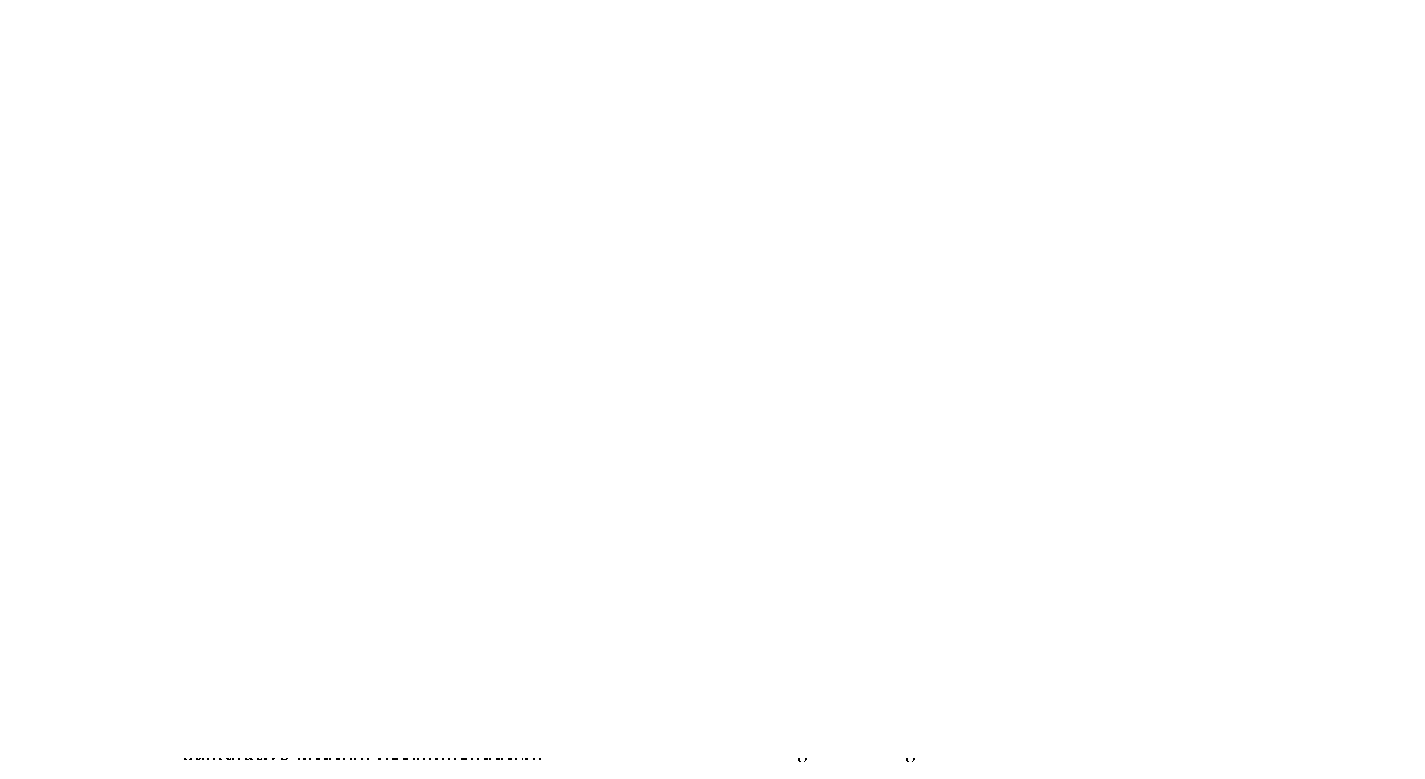
\includegraphics[width=4.5in]{./images/system.eps}
\includegraphics[width=6in]{./images/SystemBW.eps}
\vspace*{-.1in} \caption{Pipeline Design }\label{fig:system}
\vspace*{-.2in}
\end{figure}

\section{System Overview}

In this section, we sketch out the main components of the system. Our system is built with a pipeline architecture in mind which gives it the advantage to run each section separately and allow stream processing without resources being wasted by one operation while others are awaiting (Figure \ref{fig:system}). This consists of a section to perform pre-processing to prepare the required data, Cumulative Citation Recommendation to annotate cite-worthy documents, Streaming Slot Filling which generates the actual slot values and Post processing to increase precision/recall. 

%\ceg{Discuss current system first. If you want to keep the decisions points that led to the current architecture, make it a subsection.}

\subsection{Preprocessing}

To begin, we need to have real-world aliases of entities of interest. TREC KBA prohibits Wikipedia entities to have any manual aliases being added and only allows automatic ways. We use Wikipedia API backlink references (redirects to a wiki entity) as aliases of the entity. We also use some techniques to extract  aliases from within the text of a wiki entity, which will be described later on. This whole process is referred to as \textit{Alias Extraction (Wiki API, Wiki text)}. On the other hand, regarding Twitter entities this limit is lifted and participants are allowed to manually add aliases for them. Part of the reason is that Twitter environment is composed of so much informal and dialectic language which makes it extremely difficult to extract alias out of tweets or entities descriptions in their profiles. This process of extracting aliases for Twitter entities is referred to as \textit{Manual Alias Extraction (Twitter)}.

Once aliases are available we pass them through some rules of generating proper name orders which will produce various forms of writing a name. As a basic example Bill Gates can be written as Gates, Bill. This will allow the system to capture various notation forms of aliases. We refer to this part as \textit{Name Order Generator}.

\subsection{CCR}

The main goal of Cumulative Citation Recommendation is to have an aggregate list of documents that are worthy of being cited in a Wikipedia page. Regarding CCR we perform exact string matching 
and treat all the documents that mention an entity equally likely to be citable.
For future iterations of the paper we have ideas on how to score documents 
based on their likelihood of citation worthiness, but for this iterations we 
treat all mentioning documents equally likely. One of the reasons for this is 
that in former TREC KBA reports \cite{JFrank12} there were observations of how 
non-mentioning documents have highly low chance of being citable in Wikipedia.
So we take on that and ignore non-citing documents. Regarding mentioning but 
garbage, neutral or central documents we produce more slot values which can be 
later on filtered out in the high accuracy filter section.

Our pipeline of processing the corpus consists of a two layer indexing system referred to as \textit{Chunk Files Index Generator} and \textit{StreamItems Index Generator}.  Chunk Files Index Generator will generate indexes of the chunk files that contain a mention of any of the desired entities. StreamItems Index Generator on the other hand will index StreamItems that contain a mention of a given entity respectively. This two level indexing will eliminate the need to process each and every ChunkFile/StreamItem for every entity. 



% Note: Describe the algorithms of each phase
% Talk in abstract terms not implementation.
% Use formal representations (Math, SQL etc)


%\ceg{This section should be structured as follows:
%1: Introduce CCR (Motivation, Expectations)
%2: Our high level approach
%3: Discussion of our design (Like already discussed)
%}


\subsection{SSF}
%\ceg{See the previous note.}
As described in the Introduction, the general purpose of slot filling is to extract proper values for relations of interest, some of which can be found in Table \ref{table:slotNameOntology}. This is called Stream Slot Filling due to the fact that it is assumed that data is being generated as time goes on and for each extraction we should only consider current or past data. In our schematic diagram we refer to this as \textit{Streaming Slot Value Extraction}. Stream slot filling is done by pattern matching documents with manually 
produced patterns for slots of interest. The way we do this is by observing a 
sentence that has a mention of the entity or one of its coreferences. An 
anchor word in the sentence related to the slot name is located and we match 
either left or right of the anchor word for potential slot values. 

\subsection{Post Processing Algorithm}

The SSF output of many extractions is noisy. The data contains duplicates and 
incorrect extractions. We can define rules to sanitize the output only using 
the information present in the SSF file. The file is processed in time order, 
in a tuple-at-a-time fashion to minimize the impact on accuracy. We define 
two classes of rules deduplication rules and inference rules. In our diagram we refer to this component as \textbf{High Accuracy Filter}.
